\chapter{Free-Free contamination}
\label{ch:chapter4}

%W40 - intro preamble 
In this chapter we examine the arguments for a thermal Bremsstrahlung, or free-free, 
contribution to the SCUBA-2 detections, addressing questions regarding the source, 
strength, spectral index, and location of the turnover (from partially opaque to optically 
thin) of free-free emission. We examine the various sources of free-free emission in 
the JCMT GBS and asses the magnitude of the contribution of free-free to SCUBA-2 
bands.

\section{Introduction to thermal breemstralung emission}

%NEW - background theory
Thermal Bremsstrahlung, or free-free, emission is a thermal process by which photons are produced from electron scatter in a plasma in LTE. We derive the spectral index of the free-free emission by first considering the number of electrons, $N_{e}$, passing an ion, per unit time. The electrons have a speed range $v$ to $v + dv$ and the the ion has an impact parameter of $b$ to $b + db$ such that 
\begin{equation}
N_{e}(2\pi b\,db)vf(v)\,dv. \label{eqn:ion}
\end{equation}
In this system the number of `encounters', $N(v,b)$, between the ion and an electron, per unit volume, per unit time, is 
\begin{equation}
N(v,b)\,dv\,db = (2\pi\,db)[vf(v)]N_{e}N_{i}, \label{eqn:encounters}
\end{equation}
and the average energy per unit frequency, $W_{\nu}$, is 
\begin{equation}
W_{\nu}\approx \frac{\pi^{2}}{2}\frac{Z^{2}e^{6}}{c^{3}m_{e}^2}\left ( \frac{1}{b^{2}v^{2}} \right ) 
\label{eqn:energy}
\end{equation}
where the above constants have their usual meanings. From radiative transfer, the emission coefficient, $\epsilon _{\nu}$, can be calculated by integrating energy and encounters over $b$ and $v$ as such, 
\begin{equation}
4\pi\epsilon _{\nu}=\int_{b=0}^{\infty }\int_{v=0}^{\infty }W_{v}(v,b)N(v,b)\,dv\,db. \label{eqn:epsilon} 
\end{equation}
Considering non-relativistic Maxwellian distribution of electron velocities,  
\begin{equation}
f(v)=\frac{4v^{2}}{\sqrt{\pi }}\left ( \frac{m_{e}}{2k_{B}T_{e}} \right )^{3/2}exp\left (- \frac{m_{e}v^{2}}{2k_{B}T_{e}} \right ), \label{eqn:max}
\end{equation}
the free-free emission coefficient can be derived as 
\begin{equation}
\epsilon _{\nu}=\frac{\pi^{2}Z^{2}e^{6}N_{e}N_{i}}{4c^{3}m_{e}^{2}}\left ( \frac{2m_{e}}{\pi\,k_{B}T_{e}} \right )^{1/2}ln\left ( \frac{b_{max}}{b_{min}} \right ).
\label{eqn:eff}
\end{equation}
The minimum and maximum impact parameters, $b_{min}(v)$ and $b_{max}(v,\nu)$, make up the Gaunt factor, 
\begin{equation}
g_{ff}(\nu,T) = \frac{\sqrt{3}}{\pi}ln\left (\frac{b_{max}}{b_{min}} \right), 
\label{eqn:gaunt}
\end{equation}
that value of which ranges as $g_{ff}(\nu)\propto 1/\nu$ between 1 and 10 across the radio spectrum. Using Kirchoff's law ($\kappa_\nu=\epsilon_{\nu} / B_{\nu}(T)$) the absorption coefficient, $\kappa_\nu$, can be calculated in the Rayleigh-Jeans limit as 
\begin{equation}
\kappa_\nu=\frac{1}{\nu^{2}T^{3/2}}\frac{\pi^{3}}{\sqrt{48}}\,g_{ff}\left [ \frac{Z^{2}e^{6}}{c}N_{e}N_{i}\frac{1}{\sqrt{2\pi\,(m_{e}k_{B})^{3}}} \right ].
\label{eqn:kappaff}
\end{equation}
Because the Gaunt factor is weakly inversely proportional to frequency the opacity of free-free emission can be approximated to $\kappa_\nu \propto \nu^{-2.1}$ \citep{Oster:1961fk, Altenhoff:1970ai} and as a result the optical depth of the free-free can be written as 
\begin{equation}
\tau_\nu \approx \int \frac{N_{e}^{2}}{\nu^{2.1}T^{3/2}}\,ds.
\label{eqn:Tauff}
\end{equation}
From this expression it can be determined that at low frequencies $\tau_\nu \gg 1$ and emission will become optically thick. Likewise at very high frequencies emission will become optically, $\tau_\nu \ll 1$. Considering the equation of flux density from radiative transfer, 
\begin{equation}
S_\nu= \int_{\Omega }B_{\nu}(T,\nu)\tau\,d\Omega, 
\label{eqn:Snu}
\end{equation}
it is possible to show that free-free emission at very low frequencies will resemble a black body where $S_\nu \propto \nu^{2}$. Likewise at very high frequencies free-free emission is approximately flat, $S_\nu \propto \nu^{-0.1}$ \citep{Mezger:1967fk}.

%NEW-turnover
At $\tau_\nu = 1$ free-free emission will undergo a `turnover' from the optically thick to thin regime, typically at low frequencies around KHz regime.  At very high frequencies another break occurs in the spectrum when $h\nu \gg k_{B}T_{e}$ and the free-free spectrum goes from flat to an exponential decay that is described by, 
\begin{equation}
J_{\nu,T} \propto T^{-1/2}exp\left ( \frac{-h\nu}{k_{B}T_{e}}\right) N_{e}^{2} g_{ff}(\nu,T), 
\label{eqn:expdecay}
\end{equation}
where $J_{\nu,T}$ is the emissivity [CITE]. For a electron temperature of $10^{4}$\,K, the exponential decay break can be estimated at occurring short ward of 1\,$\micron$. 

\section{\HII\ observations}
%W40
\begin{figure}
\begin{centering}
\includegraphics[scale=0.5]{/Users/damian/Documents/Thesis_et_al/Papers/starformation_in_W40/W40images/20150904_W40Hiiregion.pdf}
\caption{Archival VLA 21\,cm NRAO VLA Sky Survey \citep{Condon:1998kx} continuum map of the W40 complex \HII region (45\arcsec\ resolution). Red  \emph{Herschel} 70$\micron$ contours of the nebulosity SH-64 at 300, 1200, 4800, 12000\,MJy/Sr. Blue SCUBA-2 850\,$\micron$ 
contours of the dust cloud at the 5$\sigma$ level. Yellow stars indicate the locations of the OB stars, with the O9.5 star OS1 the primary ionising object of the region. The white cross indicates the peak of the VLA 21\,cm emission.} 
\label{fig:21cm}
\end{centering}
\end{figure} 

%NEW - lyman photons
In star formation, free-free emission is typically observed from H\,\textsc{ii} regions formed by photoionisation of molecular hydrogen by UV photons from B4V stars or earlier. The UV, or Lyman, photon density, $N_{Ly}$,  required to maintain the ionisation of an \HII\ region is given by \cite{Kurtz:1994cr} as 
\begin{equation}
N_{Ly} \geq 8.04\times10^{46}T_{e}^{-0.85}U^{3}, 
\label{eqn:lyman}
\end{equation}
where U is the excitation parameter $R_{s}N_{e}^{2/3}$ for a Stromgern sphere of radius $R_{s}$. These two variables are also related through 
\begin{equation}
N_{Ly} = \alpha _HN_e^{2}\frac{4}{3}\pi\,R_s^3
\label{eqn:stromgern}
\end{equation}
where $\alpha _H$ is the hydrogen recombination rate, approximately equal to 3$\times$10$^{-13}$\,cm$^{3}$\,s$^{-1}$. \HII\ regions are large scale, low density structures with radii greater than $10^{18}$\,cm and $N_{e}$ less than $10^{4}$\,cm$^{-3}$. The stellar $N^{*}_{Ly}$ for the OB stars capable of producing \HII\ regions is typically greater than $10^{46}$\,cm$^{-3}$. By considering $N^{*}_{Ly}$ at specific frequencies \cite{Kurtz:1994cr} calculates the flux density that would be observed if viewing an \HII\ region at a distance, $d$, using 
\begin{equation}
S_{\nu}(\mathrm{Jy}) = 1.32\times10^{-49}\xi N^{*}_{Ly}a(\nu,T)\left ( \frac{\nu}{\mathrm{GHz}} \right )^{-0.1}\left ( \frac{T_{e}}{\mathrm{K}} \right )^{0.5}\left ( \frac{d}{\mathrm{kpc}} \right )^{-2},
\label{eqn:kurtz}
\end{equation}
where a$(\nu,T)$ is a constant equal to 0.98 \citep{Mezger:1967fk} and $\xi$ is the fraction of UV photons not absorbed by the dust set at 10\%. Free-free emission from large scale, diffuse H\,\textsc{ii} regions is predicated to be optically thin at radio frequencies emission where the power law becomes approximately flat with an $\alpha_{\mathrm{ff}}$ = -0.1 \citep{Oster:1961fk, Mezger:1967fk}. 

%\NEW - general info on Hii regions
In an \HII\ region UV heat up the gasses and plasma of the ISM by radiative transfer to temperatures in excess of 10000\,K. This causes the exposed material to expand adiabatically into the space surround the OB star/s. In the transition zone between the \HII\ region and the neutral ISM two fronts are observed; the ionisation front [CITE] and the shock [CITE]. In the shock front, expansion of the \HII\ region is thought to sweep up the ISM producing localised over densities associated with a `shell' of material around the \HII\ region [CITE]. Whether the shock front has sufficient pressure to destabilise existing cores within any exposed filaments and `trigger' star-formation is an open question \citep{Lefloch:1994uq, Urquhart:2009dq}. The ionisation front represents a region where neutral material is being ionised through exposure to UV photons. Rate of ionisation is heavily dependant on the local density. High density regions take considerably longer to break down than lower density regions and as a result `champagne' flows \citep{Dale:2012fk} are observed where the molecular cloud has been ruptured by an internal \HII\ and photons are exiting through a narrow opening. The \HII\ region can be further imbedded by accretion flow of neutral material onto the star \cite{Dale:2005kx, Dale:2011vn} and by gravity when at the centre of massive cloud \cite{Yorke:1989ys}. The region in-between the ionisation front and shock front is collectively known as a photo-dissociative region (PDR, \citeauthor{Thompson:2004uq} \citeyear{Thompson:2004uq}). An example of a PDR is observed in Perseus, a star forming region observed as part of the JCMT GBS.   

\section{\UCHII\ observations}

 %W40
\begin{figure*}
\begin{centering}
\begin{tabular}{l}
\includegraphics[scale=0.28]{/Users/damian/Documents/Thesis_et_al/Papers/starformation_in_W40/W40images/free-free-alpha-sketch.pdf}
\includegraphics[scale=0.28]{/Users/damian/Documents/Thesis_et_al/Papers/starformation_in_W40/W40images/20150506_freefreecutoff.pdf}
\end{tabular}
\caption{\textbf{Left]} A schematic of the SED shape for three hypothetical scenarios of{fig:freefreealpha} free-free emission. %\\
\textbf{Case a)} an UCH\,\textsc{ii} with $\alpha_{\mathrm{ff}}$ = 0.6 has a turnover that occurs short ward of the submillimetre regime, and as a result has a majority contribution to the 850\,$\micron$ band and a significant contribution to the 450\,$\micron$ band. %\\
\textbf{Case b)} a YSO emits free-free emission, $\alpha_{\mathrm{ff}}$ = 1.0, from a collimated jet. However the spectrum turns over to the optically thin regime long ward of submillimetre wavelengths, and consequently free-free emission contributes roughly equally to both SCUBA-2 bands. %\\
\textbf{Case c)} a H\,\textsc{ii} region has free-free emission from diffuse gas of $\alpha_{\mathrm{ff}}$ = -0.1 that outshines that from compact objects at long wavelengths. However, the flat spectrum means that at submillimetre wavelengths the emission is all but negligible.
\textbf{Right]} Free-free turnover as a function of launching electron density (as described by \citeauthor{Olnon:1975bh} \citeyear{Olnon:1975bh}  in Equation \ref{eqn:turnover}). Dashed lines indicate the submillimetre regime (1.3\,mm to 350\,$\micron$).}
\label{fig:freefreealpha}
\end{centering}
\end{figure*} 

%W40 - uchii scale intro
In addition to these large scale structures, free-free emission is also detected in the form of a power law at scale sizes comparable to individual stars \citep{Panagia:1975uq}. 

%NEW - what is an UCHII
Early type OB stars undergoing mass loss through winds produce free-free emission from ionised material leaving the star, in addition to UV photons ionising the ISM, and are considered compact ($\leq$0.5$\hbox{ pc}$), ultra compact ($\leq$ 0.1$\hbox{ pc}$) and hyper compact ($\leq$ 0.03$\hbox{ pc}$) \HII\ regions \citep{Wright:1975kx, Harvey:1979qf}. These are the processors of evolved \HII\ regions (10$\hbox{ pc}$,\citeauthor{Kurtz:2005kl} \citeyear{Kurtz:2005kl}). From here on in we refer to these classes collectively as \UCHII\ regions. Whereas \HII\ regions are diffuse, homogenous fields of emission, \UCHII\ regions have an electron density is inversely proportional to radius. Assuming spherical winds of constant velocity \cite{Panagia:1975uq} and \cite{Wright:1975kx} derive the spectral index of the free-free emission as $\alpha_{\mathrm{ff}}$ = 0.6. Large surveys of \UCHII\,candidate regions are consistent with this result \citep{Harvey:1979qf, Wood:1989bh, Kurtz:1994cr, Molinari:1998dq, Walsh:1998nx, Kurtz:2005kl}.

%W40 - EDIT - turnover equ
Where the free-free emission mechanism is a spherical ionised stellar wind,Emission can be thought of as \emph{partially thick} with lower frequencies probing greater depths of emission within the wind before becoming fully optically thin at shorter wavelengths where only the diffuse \HII\ region is being observed. The exact location of this free-free turnover, $\nu_{c}$, has been much debated in the literature. If the turnover occurs short-ward of submillimetre wavelengths then it is possible that the free-free may contribute in part to SCUBA-2 observations of dust emission. \cite{Olnon:1975bh} defines $\nu_{c}$ as a function of electron density, N$_{e}$(R) = N$_{e,0}$ where r $\leq$ R, as 
\begin{equation}
\log_{10} \nu _{c} = - 0.516 + \frac{1}{2.1}\log_{10}\left ( \frac{8}{3}RN_{e,0}^{2}T_{e}^{-1.35} \right ),  
\label{eqn:turnover}
\end{equation}
where R is the launching radius of the wind (typically 10\,AU) and $T_{e}$ is the electron temperature (typically 10$^{4}$\,K). Figure \ref{fig:turnover} highlights how a turnover point short wards of the submillimetre regime requires an electron density in excess of 10$^{8}$\,cm$^{-3}$. 

%W40 - electron density expression 
The electron density n$_{0}$ is not easily determined from observations. We therefore turn to indirect measurements to make a general statement about what systems will produce free-free emission that is opaque at submillimetre wavelengths and hence may subsequently be contributing to SCUBA-2 emission. We assume that n$_{0}$ is proportional to stellar mass and by association varies with spectral class as the more massive stars are known to produce more vigorous winds and greater mass loss. \cite{Sandell:2011dz}'s results indicate that the free-free contribution is significant for early B stars in their sample, but not for late B and A class stars. MWC 297 is the lowest mass star in their sample for which free-free contributes at SCUBA-2 wavelengths and we therefore mark it as a lower limit of stellar class. MWC 297 has a luminosity of 3 $\times$ 10$^{3}$\,L$_{\odot}$ \citep{Drew:1997qf} which corresponds to a class B1.5Ve or B4V star. Given the nature of these assumptions, we are limited to assigning an upper estimate of spectral class B4V, above which the free-free turnover can occur in the submilimetre regime. 

%MWC297 - uchii summarise
\UCHII\ are associated with stars that are sufficiently massive (greater than 8$M_{\mathrm{\odot}}$) that their Kelvin-Helmholtz contraction timescale is shorter than their free fall and accretion timescale \citep{Manoj:2007ly}. These stars reach the main sequence and start producing ionising radiation whilst still embedded within their protostellar envelope \citep{McKee:2003ys}. This would then lead to a compact region of highly ionised winds, as detected by \cite{Malbet:2007zr} and \cite{Drew:1997qf}. We follow \cite{Wood:1989bh}'s description of an UCH\,\textsc{ii} region as region with electron density greater than 10$^{4}$\,cm$^{-3}$ within a diameter of less than 0.1\,pc. The minute size of the \UCHII\ region means they cannot be detected optically and are interest observed through free-free processes or the indirect heating of dust. The lifetime of the ultra-compact stage of an \HII\ region is estimated at 4$\times$10$^{5}$\,years, approximately 10\% the lifetime of a typical O star. 

\begin{figure}
\begin{centering}
\includegraphics[scale=0.4]{/Users/damian/Documents/Thesis_et_al/Papers/starformation_in_W40/W40images/20150904_freefree_small.pdf}
\caption{Archival AUI/NRAO 3.6\,cm map of the W40 complex OB association (NRAO/VLA Archive Survey, (c) 2005-2007). SCUBA-2 850\,$\micron$ contours of dust emission at 5$\sigma$, 15$\sigma$ and 50$\sigma$ overlaid. Yellow markers indicate the locations of the OB stars while cyan circles indicate the location of compact radio sources identified by Rodriguez et al 2010. Cyan crosses mark the four peaks identified separately in the AUI/NRAO 3.6\,cm map.}
\label{fig:3_6cm}
\end{centering}
\end{figure} 


\subsection{Jets}

%NEW - intro jets
A minority of radio bright young OB stars are observed with $\alpha_{\mathrm{ff}} \geq$ 0.6, for example MWC 349 \citep{Olnon:1975bh}, MWC 297 \cite{Skinner:1993bh, Sandell:2011dz} and AB Aur \citep{Rodriguez:2014zr}.
%W40
\cite{Reynolds:1986cr} provides a comprehensive examination of models for stellar winds and finds that, where the outflow is highly collimated and accelerating (as this the case of bi-polar jets) the spectral index becomes increasingly opaque with $\alpha_\mathrm{ff} \simeq$ 1.0. [CAN DERIVE IF NECESSARY BUT ITS PRETTY OVERKILL].

%W40 - example jet source
MWC 349 \citep{Tafoya:2004ly,Sandell:2011dz} and MWC 297 \citep{Sandell:2011dz, Rumble:2015vn} 
are early B-class Herbig stars where empirical observations have suggested that the free-free emission 
is sufficiently bright and opaque that it dominates over the dust emission at submillimetre wavelengths 
and produces a distinct point source in the observations consistent with a compact object. If similar 
point sources are present the SCUBA-2 observations of W40 complex, and are also consistent the 
location of whole compact radio sources, that could well signify the potential for free-free contribution.


%%%%%%%%

\section{Free-free contribution to SCUBA-2}

\begin{figure}
\begin{center}
\includegraphics[scale=0.45]{/Users/damian/Documents/Thesis_et_al/images/20140821_mwc297_free_free_SED.pdf}
\caption{The Spectral Energy Distribution of MWC 297 from submillimetre to radio wavelengths. SCUBA-2 fluxes (found using aperture photometry as described in Section 5.2.) are presented alongside those collated by \protect\cite{Sandell:2011dz} who fit a power law $\alpha = 1.03\pm0.02$, consistent with free-free emission from an UCH\textrm{II} region and polar jets or outflows.}
\label{fig:freefreeSED}
\end{center}
\end{figure}

%NEW - free-free contrib intro 
Where free-free emission is significantly bright and remains optically opaque up to submillimetre wavelengths it may be detected by SCUBA-2 in the 450 and 850\,$\micron$ bands.  

%W40 - examples of turnover issue
\cite{Harvey:1979qf}, \cite{Kurtz:1994cr} and \cite{Sandell:2011dz} present multi-wavelength radio surveys of numerous HAeBe systems. A number of A class and late B class stars have faint free-free \UCHII\ detections that appear to become optically thin long-ward of the submilimetre regime or are otherwise negligible when compared to emission at from the dust in the protostellar disc or envelope. \cite{Rodriguez:2014zr} finds evidence that free-free emission in AB Aur has index $\alpha_{\mathrm{ff}}$ = 1.1 at cm wavelengths, however flux becomes optically thin by 1.3\,mm, leading to the conclusion that  $\nu_{c} \sim$ 70\,GHz. The early B systems of MWC 349, MWC 279 and LkH$\alpha$ 101 are observed to have strong free-free wind or jet emission which fits a power law right up to the submillimetre where the free-free provides a substantial, if not the majority of emission at these wavelengths. \cite{Olnon:1975bh} calculates that $\nu_{c} \sim$ 575\,GHz for MWC 349 using Equation \ref{eqn:turnover}, given that R $\sim$ 11\,AU and N$_{e,0}$ $\sim$ 9$\times$10$^{8}$\,cm$^{-3}$ \citep{Greenstein:1973uq}. \cite{Harvey:1979qf} goes further and argues that free-free emission may be opaque up to 100\,$\micron$.

We present our methods for calculating and subtracting the free-free contribution from SCUBA-2 data published in  \cite{Rumble:2015vn} and Rumble et al. (2016, in prep.). 

\subsection{Direct methods}

\begin{figure*}
\begin{center}
\includegraphics[scale=0.5]{/Users/damian/Documents/Thesis_et_al/Papers/Starformation in MWC297/mwc297_arXiv/MNRAS/20140618_mwc297_contamination.jpeg}
\caption{IR1 SCUBA-2 850\,$\micron$ data before \emph{left} and after \emph{right} removal of free-free contamination from an UCH\textrm{II} region and polar jets/winds (represented by the point source contours in the \emph{left} plot). SCUBA-2 contours are at 0.011, 0.022, 0.033 and 0.055 Jy/pixel (corresponding to 5, 10, 15 and 25 $\sigma$ detection limits). 6\,cm VLA contours (red) from Sandell (private comm.) at 0.002, 0.005, 0.02, 0.072, 0.083 Jy/beam are overlaid on the left hand panel. The location of MWC 297 is marked with a star. Beam sizes are shown at the bottom of the image (VLA CnD config. \emph{left} and JCMT \emph{right}.) }
\label{fig:contamination}
\end{center}
\end{figure*}


%MWC 297 - MWC297
\cite{Skinner:1993bh} studied free-free 3.6\,cm and 6.0\,cm radio emission from stellar winds around the B1.5ve star MWC 297 and found a power law of the form $S_{\nu} \propto \nu^{\alpha}$ where $\alpha$ is equal to 0.6238 in the optically thin regime. \cite{Sandell:2011dz} extended the study down to 3 mm and revised the spectral index to $\alpha = 1.03\pm0.02$ which is consistent with a collimated jet component to free-free emission. The free-free power law extends into the submillimetre spectrum; however, at wavelengths shorter than 2.7\,mm there is potential for a thermal dust component in the observed flux, so submillimetre flux is not included in the calculation of $\alpha$.

%MWC 297 - VLA observations
Figure~\ref{fig:contamination} displays 6\,cm radio emission from the VLA CnD configuration in conjunction with 
SCUBA-2 850\,$\micron$ data (Skinner \citeyear{Skinner:1993bh}, Sandell priv. comm). Both sets of data show 
peaks in emission which are coincident with a point source at the location of the star MWC 297 in 1\,mm and 
3\,mm data presented by \cite{Alonso-Albi:2009ve}. The peak of the SCUBA-2 850\,$\micron$ emission in 
Figure~\ref{fig:contamination} is 86\,mJy/pixel, consistent with the SCUBA 850\,$\micron$ value of 82\,mJy/pixel 
\citep{Alonso-Albi:2009ve}.

 %MWC 297 - jets obs.
The VLA data also show extended emission to the north and south of MWC 297 which is consistent with polar 
winds or jets. The intensity of emission is significantly weaker than that of the UCH\textrm{II} region. Considering 
the elongated beam shape of the VLA CnD observations (21.1\arcsec $\times$ 5.2\arcsec, PA$ = -61^{\circ}.3$) 
accounts for much the E/W elongation of the emission. In addition to this, \cite{Manoj:2007ly} describe this emission 
as coming from within 80\,AU of MWC 297. This is much smaller than the JCMT beam and therefore we model the 
dominant free-free emission from MWC 297 as a point source.

%MWC 297 - model and subtraction
By taking the revised power law least square fit to \cite{Skinner:1993bh} and \cite{Sandell:2011dz}'s results at radio and millimetre wavelengths and extrapolating to the submillimetre wavelengths of SCUBA-2, we are able to calculate the effect of free-free emission due to a point-like UCH\textrm{II} region as an integrated flux of 934$\pm$128 mJy at 450\,$\micron$ and 471$\pm$62 mJy at 850\,$\micron$. 
%NEW
Single pixels with these values were then implanted into blank SCUBA-2 450 and 850\,$\micron$ PONGs and the map convolved with the JCMT beam to produce an SCUBA-2 free-free emission map. These are subtracted off of the original SCUBA-2 maps to leave a SCUBA-2 dust map.

%NEW - large scale intro
In addition to small scale free-free structures that are modelled as point sources, we can also run a free-free subtraction for large-scale emission from the diffuse emission from the \HII\ region.

%W40 - large-scale observations
Archival VLA 21\,cm data (45\arcsec\ resolution) is presented in Figure \ref{fig:21cm} and shows the location of the 1.7\arcmin\ large scale \HII\ region associated with SH-64 \citep{Condon:1998kx}. \cite{Rodney:2008ij} presents a summary of observations at multiple radio wavelengths and conclude a flat spectral index ($\alpha$ = -0.1) as expected from homogenous, optically thin free-free emission as predicted by \cite{Oster:1961fk} and \cite{Mezger:1967fk}.  

%NEW - large-scale method
Using a simple gaussian we convolve the SCUBA-2 850\,$\micron$ up to the 45\arcsec\ resolution of the VLA data so the fluxes are comparable. Likewise we re-grid the data on to a common pixel size. SCUBA-2 data has large scale structure greater than 5\arcmin\ removed during the data reduction process so we use the \textsc{findback} tool (see Section 2) to mimic the process on the VLA data. The VLA fluxes are subsequently scaled up to 850\,$\micron$ following an $\alpha$ = -0.1 before they are subtracted from the SCUBA-2 observations. 

\begin{figure*}
\begin{centering}
\includegraphics[scale=0.65]{/Users/damian/Documents/Thesis_et_al/Papers/starformation_in_W40/W40images/20150904_freefree_large_contribution.pdf}
\caption{The free-free contribution from large-scale \HII\ gas, modelled using archival VLA 21\,cm observations \citep{Condon:1998kx} assuming $\alpha_{\mathrm{ff}}$ = -0.1 (right), compared to SCUBA-2 dust emission at 850\,$\micron$ (left). Maps have common 15\arcsec\ pixels and 45\arcsec\ resolution. Markers indicate the locations of the OB stars.} 
\label{fig:freefree21}
\end{centering}
\end{figure*} 



\subsection{Indirect methods}

%W40
\begin{table*}
\caption{Summary of radio findings on bright objects in W40. }
\begin{center}
\begin{tabular}{|ccccccccc|}
\hline
Source	&	2MASS ID		&	Type		&	Time				&	Associated	&	SCUBA-2 		&	Free-free		&	Proposed				&	Distance  \\
		&				&			&	variable 3.6\,cm?	&	jet?			&	point source?	&	optically thick?	&	$\alpha_{\mathrm{ff}}$		&	(pc)		\\
\hline
\hline
OS 1a (North)	& 18312782-0205228	& 	Herbig AeBe	&	N	&	N	&	Y	&	?	&	0.6	&	536$^{+42}_{-95}$	\\
OS 1a (South)	& 18312782-0205228	&	O9.5			&	-	&	N	&	Y	&	-	&	-	&	536$^{+42}_{-95}$	\\
OS 1b		& 18312866-0205297	&	Class II		&	N	&	Y	&	N	&	N	&	-0.1	&	-				\\
OS 1c		& 18312601-0205169	&	Class II		&	Y	&	N	&	N	&	N	&	-0.1	&	-				\\
OS 2a		& 18312397-0205295	&	Herbig AeBe	&	Y	&	?	&	Y	&	?	&	1.0	&	-				\\
OS 2b		& 18312257-0205315	&	B4			&	Y	&	N	&	Y	&	?	&	-0.1	&	455$^{+71}_{-59}$	\\
OS 3a		& 18312395-0204107	&	B3*(binary)	&	-	&	-	&	N	&	-	&	-	&	454$^{+87}_{-48}$	\\
IRS 5		& 18311482-0203497	&	B1			&	-	&	-	&	N	&	N	&	-0.1	&	469$^{+217}_{-129}$	\\
\hline
\end{tabular}
\end{center}
\label{tab:stars}
\end{table*}%

\begin{figure*}
\begin{centering}
\includegraphics[scale=0.6]{/Users/damian/Documents/Thesis_et_al/Papers/starformation_in_W40/W40images/20150904_W40_freefree_comb.pdf}
\caption{The free-free contribution of compact radio sources OS1a and OS2a at 450\,$\micron$ (left) and 850\,$\micron$ (right), modelled as point sources extrapolated from the Rodriguez et al. 2010 3.6\,cm fluxes with assumed spectral indices given in Table \ref{tab:freefree}. Yellow markers with thick outlines indicate the locations of the OB stars, cyan circles the location of all the Rodriguez et al. 2010 compact radio sources and cyan crosses the location of four peaks identified separately in the AUI/NRAO 3.6\,cm map (450\,$\micron$ only). Black contours trace SCUBA-2 data at 3$\sigma$, 5$\sigma$, 15$\sigma$ and 30$\sigma$. Red and green filled contours trace the free-free contribution at 3$\sigma$ and 5$\sigma$ from optically thick (see Table \ref{tab:stars}).} 
\label{fig:freefree3_6}
\end{centering}
\end{figure*} 

%NEW - intro indirect methods
In the previous section we were able to combine observations across a range of wavelengths to directly and accurately calculate the free-free spectral index. Other regions have been less well studied in high resolution and radio catalogues exist only for single wavelengths from which it is not possible to directly calculate $\alpha_{\mathrm{ff}}$. In order to get around this problem we can asses the radio properties of any free-free sources to determine whether or not it can be classified as \HII, spherical wind \UCHII or collimated jet \UCHII\ region. By considering the spectral class (if known) of the source and SCUBA-2 observations we can also make a judgement on whether or not any free-free emission is optically thick or thin at submillimetre wavelengths. In this way we can indirectly estimate the extent the free-free contribution to SCUBA-2 observations in more regions.

In the W40 complex 
%W40 - VLA observations/catalogues
archival AUI/NRAO 3.6\,cm data is used and presented in Figure \ref{fig:3_6cm}. The coverage of this region is limited approximately 5\arcmin\ and resolution of 9.97\arcsec\ is comparable to SCUBA-2. As a result AUI/NRAO 3.6\,cm is not able to resolve individual sources but can pick up extended radio emission associated with outflows. \cite{Rodriguez:2010bs} supplement these data with high-resolution photometry at the same wavelength but with a reduced coverage of 4\arcmin. 

%W40 - indirect methods
No additional observations of alternative wavelengths at comparable resolution are available to this author, therefore it is not possible to empirically measure the free-free spectral index and we turn to indirect methods to infer 
$\alpha_{\mathrm{ff}}$. 
%NEW
This requires examining the evidence for sufficient electron density, $N_e$, for any free-free emission to remain optically thick up to the submillimetre regime, and for features that hint that the host star may power a jet. 

The W40 complex contains a number of massive star and 
%W40 - bright stars and radio sources
\cite{Shuping:2012ly} conduct a NIR study of the brightest objects in W40, identifying a list of one late O star, 3 B stars, 2 Herbig AeBe stars and 2 low mass Class III YSOs. These objects are listed in Table~\ref{tab:stars} and build on early IR studies by \cite{Smith:1985bv}.  \cite{Rodriguez:2010bs} resolves 20 compact radio sources, 15 of which are consistent with 2MASS sources and, by using time-variability, is able to classify 8, variable, YSOcs and 7, non-variable, \UCHII\ candidate regions. \cite{Rodriguez:2010bs} also identify non-compact radio sources without IR counterparts and these are interpreted as shock fronts from thermal jets that were likely formed by the local HAeBe stars OS1b and OS2a/b. 

%NEW - SCUBA-2 point source test
The example early B systems of MWC 349, MWC 279 and LkH$\alpha$ 101 \citep{Sandell:2011dz} all have free-free emission that is opaque at submillimtere wavelengths which can be identified as a bright peak in SCUBA observations. The lack of a bright submillimetre point source consistent with the candidate \UCHII\ would likely signify that free-free emission turns over too early, or that emission is not bright enough to have a significant impact on the total flux density observed by SCUBA-2. This test immediately rules out OS1b, c, OS3a and IRS 5 from having significant \UCHII\  regions as they are not detected in SCUBA-2 at either wavelength. 
 
%W40 - radio character test
OS1 and OS2a, presented in Figures \ref{fig:21cm} and \ref{fig:3_6cm} have coincident SCUBA-2 emission so in these cases we make the initial assumption that 100\% of emission at SCUBA-2 850\,$\micron$ is produced by free-free and measure the subsequent spectral index. This initial assumption is subsequently adjusted until a spectral index that fitted a model of $\alpha_{\mathrm{ff}}$ $\sim$ -0.1, 0.6 or 1.0. Photometry from SCUBA-2 450 and 850\,$\micron$ and AUI/NRAO 3.6\,cm maps was conducted with a 14.5\arcsec\ aperture (the SCUBA-2 850$\micron$ beam FWHM). %NEW
\cite{Rodriguez:2010bs} also detects time variability of radio emission from a number of radio sources in the W40 complex, concluding that a variable detection is symptomatic of episodic accretion processes and non-variable emission are a result of an \UCHII\ region. They also detect a number of irregular radio without an IR detection which they interpret at shocks from jet outflows. We use these as further tools to indirectly infer whether or not a YSO has an \UCHII\ region and/or jet.

\begin{figure*}
\begin{centering}
\begin{tabular}{l}
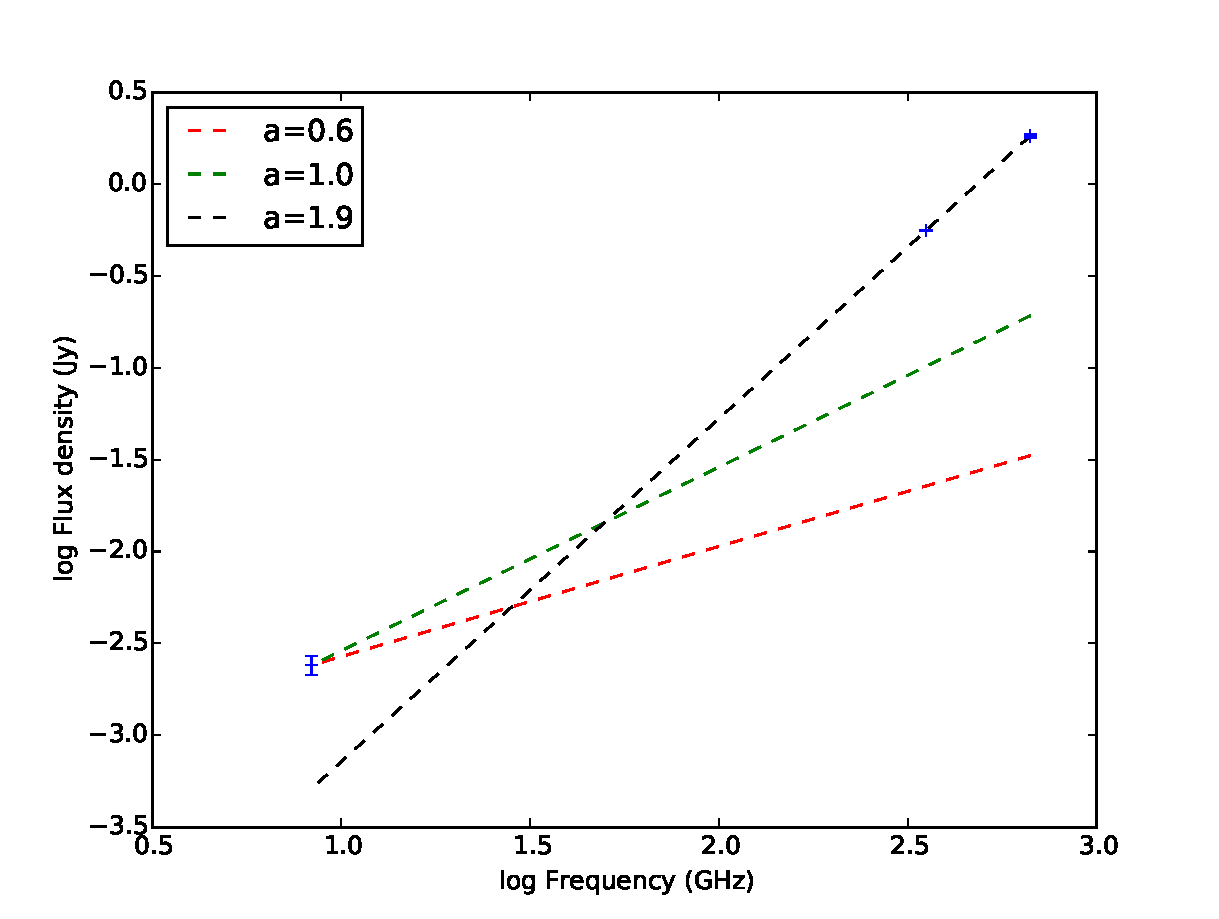
\includegraphics[scale=0.5]{c4/figs/ffOS2a.pdf}
%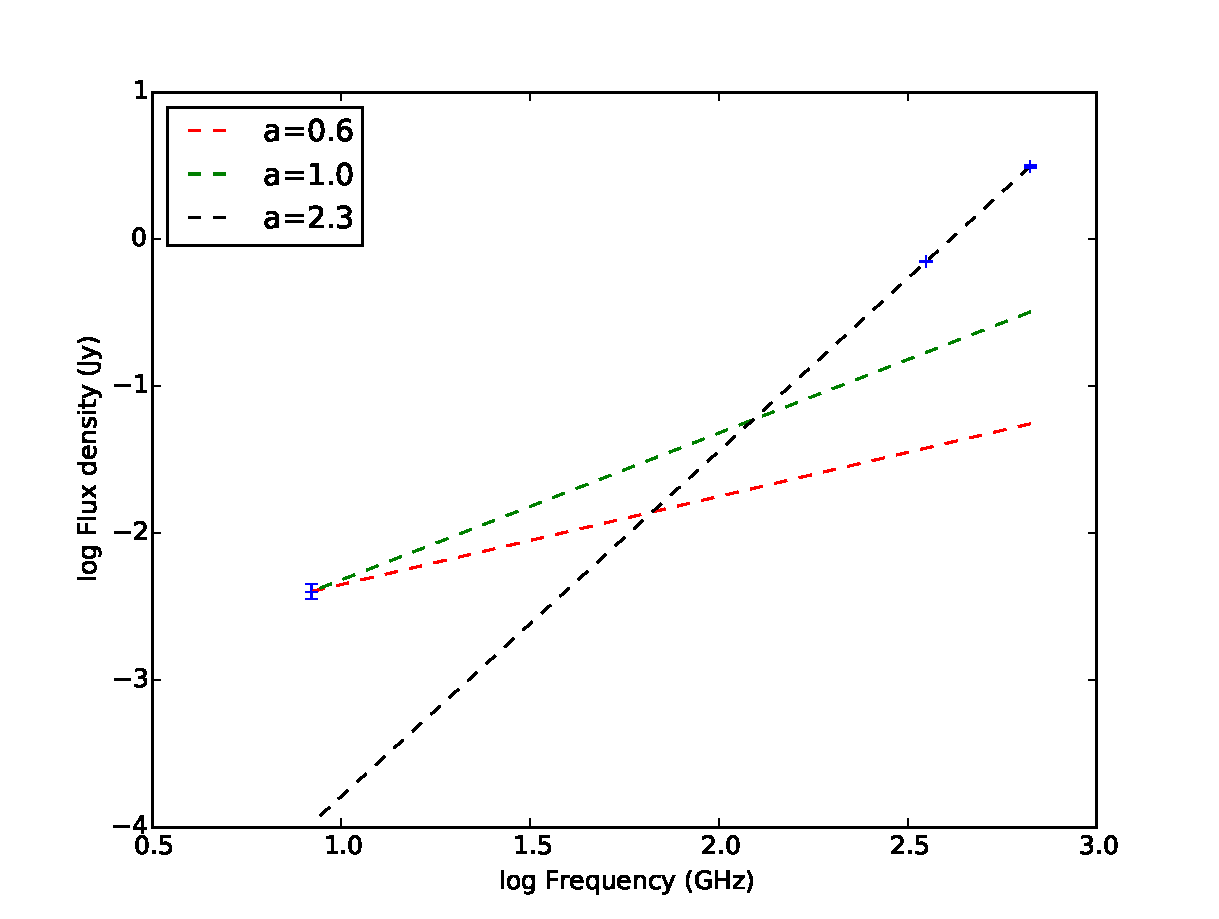
\includegraphics[scale=0.35]{c4/figs/ffOS2b.pdf}
\end{tabular}
\caption{Modelling free-free emission in OS2a from the Rodriguez et al. (2010) 3.6\,cm data for a given $\alpha_{\mathrm{ff}}$ = 0.6 (red), 1.0 (green), and the observed dust spectral index (black).} 
\label{fig:freefreemodel}
\end{centering}
\end{figure*} 

%W40 - OS1 
OS1 is a close cluster of objects that are not resolved by SCUBA-2 or the AUI/NRAO beam but are listed as a number of objects in \cite{Rodriguez:2010bs}, four of which have none-variable emission indicating an \UCHII\ region. There is also no significant emission at 450\,$\micron$ which suggests that if there is any free-free contribution at 850\,$\micron$, the emission has become optically thin by 450\,$\micron$. An $\alpha_{\mathrm{ff}}$ = 0.6 represents emission of 6.36\,mJy of free-free at 850$\micron$, a 50\% contribution. This result is consistent with the presence of HAeBe stars in the cluster. No jet shocks are found in the vicinity of the cluster and so we rule out the collimated jet configuration of free-free emission.

%W40 - OS2a
OS2a is a single HAeBe star that is resolved as a strong point source by SCUBA-2 at both 450\,$\micron$ and 850\,$\micron$. \cite{Rodriguez:2010bs} does resolve both OS2a at 3.6\,cm and therefore these fluxes are used to complete the contribution test. Two results are returned; an $\alpha_{\mathrm{ff}}$ = 0.6 represents a 5\% contribution (1.86\,mJy) and an $\alpha_{\mathrm{ff}}$ = 1.0 represents a 22\% contribution (8.18\,mJy). 
%W40 -EDIT
OS2a is variable in nature but it also has nearby shock fronts which are consistent with active accretion, so the jet scenario of $\alpha_{\mathrm{ff}}$ = 1.0 appears the more likely outcome. No spectral class is available for this object. 
Both tests infer that even if the free-free emission is opaque at SCUBA-2 wavelengths, the SCUBA-2 source is remains dominated by dust emission. These results, and others, are summarised in Table \ref{tab:stars}.
%NEW - OS2b
OS2b has a SCUBA-2 peak at both wavelengths but given its spectral class of B4 we consider it unlikely that any free-free emission will remain optically thick in the submillimetre regime. 

%W40 - VLA peaks
In addition to this radio catalogue, we identify four radio peaks in Archival AUI/NRAO 3.6\,cm map which were outside 
of the coverage of \cite{Rodriguez:2010bs} which are marked in Figure \ref{fig:3_6cm} as VLAa, b, c and d. As there is no clear point source in the SCUBA-2 maps we assume that these additional VLA radio sources are optically thin at these wavelengths and take no further action.






\section{The free-free contribution in Serpens MWC 297 results and discussion.}

%NEW
\begin{table}%[h]
\caption{Summary of free-free contributions to SCUBA-2 wavelengths from MWC 297. The uncertainty on flux density at 450\,$\micron$ is 0.03\,Jy and 850\,$\micron$ is 0.0025\,Jy. }
\begin{tabular}{@{}|c|ccccccccc|c|}
       & 3.6\,cm (Jy)	& \multicolumn{4}{c}{450\,$\micron$ (Jy)} & \multicolumn{4}{c}{850\,$\micron$ (Jy)} \\
Object &	VLA$^{a}$	& SCUBA-2       & Free-free      & Dust      & \%      & SCUBA-2      & Free-free      & Dust       & \% 	& $\alpha_{\mathrm{ff}}$     \\
\hline
\hline
MWC 297   &	0.0099	& 0.1886             &  0.1377         &  0.0510 & 73$\pm$5 & 0.0860	&	0.0709	&	0.0150	&	82$\pm$4	&	1.03      \\

\hline
\end{tabular}\\
\raggedright

\label{tab:MWC297}
\end{table}

%MWC 297 - critique free-free nature
We determine that free-free emission from an UCH\textrm{II} region and polar jets/winds associated with MWC 297 contaminates the 450\,$\micron$ and 850\,$\micron$ data \citep{Skinner:1993bh}. The nature of the free-free emission from the outflow has been debated by various authors. \cite{Malbet:2007zr} and \cite{Manoj:2007ly} argue for ionised stellar winds that dominate at higher latitudes, whereas \cite{Skinner:1993bh} and \cite{Sandell:2011dz} provide evidence for an additional source of free-free emission in the form of highly collimated polar jets. Jets are typically associated with less evolved objects where luminosity is dominated by accretion processes whereas MWC 297 is considered to be a Class III / ZAMS star where the majority of the disk has fallen onto the star or been dissipated by winds. 

%MWC 297 - Xray flares - companion 
X-ray flares are thought to be a signature of episodic accretion and \cite{Damiani:2006ve} detect a number of X-rays flares from the Serpens MWC 297 region but find that only 5.5\,per cent of total flaring is directly associated with MWC 297, suggesting that accretion onto it is minimal. The majority of X-ray emission is associated with additional YSOs and the companion of MWC 297, \emph{OSCA}, an A2V star identified by \cite{Habart:2003fk} and \cite{Vink:2005uq} at a separation of 850\,AU. 

%MWC 297 - EDIT- flux results
Figure~\ref{fig:freefreeSED} and Figure~\ref{fig:contamination} show that free-free emission due to an UCH\textrm{II} region and polar winds/jets is responsible for the majority of flux from the star MWC 297. Original peak fluxes of 188$\pm$16\,mJy and 86$\pm$22\,mJy. Residual dust peak fluxes are $51\pm10$ mJy and $15\pm3$ mJy flux per pixel at 450\,$\micron$ and 850\,$\micron$ respectively and are highlighted in Figure~\ref{fig:freefreeSED} as the flux above the free-free power law fit of $\alpha = 1.03\pm0.02$. Free-free subtraction increases the residual dust spectral index by 35\%. This corresponds to approximately 73$\pm$5\,per cent and 82$\pm$4\,per cent of the 450\,$\micron$ and 850\,$\micron$ peak flux respectively. Given our estimate of 13\,per cent CO contamination, dust emission could potentially account for as little as 5\,per cent of peak emission at 850\,$\micron$. 

%MWC 297 - dust in MWC 297?
The 5$\sigma$ level of 82\,mJy and 11\,mJy means that flux is too uncertain to be detected at 450$\micron$ and therefore it is not possible to calculate reliable temperatures of the residual circumstellar envelope/disk around the star. The assumption of point-like free-free emission may add further uncertainty to the residual flux. We cannot say whether any dust emission contributes at the position of MWC 297. 

\section{The free-free contribution in the W40 complex results and discussion.}

%W40
\begin{table}%[h]
\caption{Summary of free-free contributions to SCUBA-2 wavelengths from bright objects in W40. The uncertainty on flux density at 450\,$\micron$ is 0.017\,Jy and 850\,$\micron$ is 0.0025\,Jy. }
\begin{tabular}{@{}|c|ccccccccc|c|}
       & 3.6\,cm (Jy)	& \multicolumn{4}{c}{450\,$\micron$ (Jy)} & \multicolumn{4}{c}{850\,$\micron$ (Jy)} \\
Object &	VLA$^{a}$	& SCUBA-2       & Free-free      & Dust      & \%      & SCUBA-2      & Free-free      & Dust       & \% 	& $\alpha_{\mathrm{ff}}$     \\
\hline
\hline
OS1$^{b}$   &	0.00578	& -             & -              & -         & -       & 0.101        & 0.064          & 0.038      & 62	&	0.6      \\
OS2a   &	0.00240	& 1.83          & 0.16           & 1.67      & 9      & 0.558        & 0.069          & 0.489      & 12	&	1.0     \\
\hline
\end{tabular}\\
\raggedright
$^{a}$ VLA 3.6\,cm compact object fluxes \citep{Rodriguez:2010bs}. \\
$^{b}$ OS1 covers a cluster for stellar objects where OS1a(North), VLA-12, VLA-14, VLA-16 are all radio emitters. The flux of the most prominent source, VLA-14, is included in this table but in reality the SCUBA-2 free-free flux of OS1 is a combination of all 4 of these objects. \\
\label{tab:freefree}
\end{table}

%NEW - preamble
The W40 complex contains a number of massive stars that are detected in high resolution VLA 3.6\,cm observations. A large-scale \HII\ region is also observed at lower resolution 21\,cm observations. 

%W40 - EDIT - large-scale results
Figure \ref{fig:freefree21} shows how the SCUBA-2 data is subsequently aligned and convolved to the larger resolution of the VLA 21\,cm data so the two data sets are directly comparable. Given that free-free emission from the large scale \HII\ region is essentially flat in spectrum, it is not surprising that the contribution is very limited. Peak 21\,cm flux density is 0.0298\,Jy/pix which corresponds to 0.0163 and 0.0174\,Jy/pix at 450 and 850\,$\micron$ given a spectral index of 
$\alpha_{\mathrm{ff}}$ = -0.1. The contribution of this peak flux to the SCUBA-2 observations is 5\% at 850\,$\micron$ and 0.5\% at 450\,$\micron$. 
%NEW
As a result the dust spectral index for the peak increases by 2\% from 3.46 to 3.53.

%W40 - EDIT - small scale results
3.6\,cm fluxes for OS1 and OS2a are extrapolated up to SCUBA-2 wavelengths (Table \ref{tab:freefree}) assuming an indirectly estimated free-free spectral index of 0.6 and 1.0 respectively. Modelled as a point source, the free-free emission from each star is convolved with the JCMT beam using primary and secondary components for comparison with the SCUBA-2 data (Figure \ref{fig:freefree3_6}). The contribution of the free-free in OS1a at 850\,$\micron$ 
is 62\% (no detection at 450\,$\micron$). The free-free contribution for OS2a is 9\% at 450\,$\micron$ and 
12\% at 850\,$\micron$. 
%NEW
As a result the dust spectral index for the peak increases by 3\%.

%NEW - OS2b alpha
Having accounted for possible CO and free-free contamination, the residual flux detected from OS2a is 1.67 and 0.489\,Jy at 450\,$\micron$ and 850\,$\micron$ respectively. We find that this gives OS2a an usually low spectral index of 1.6$\pm$0.1. 
%W40
Whilst lower $\alpha$s have previous been explained by very low $\beta$ associated with grain growth \citep{Manoj:2007ly}, given a $\beta$=1.0, typical for circumstellar disks, an $\alpha$ = 1.6 would require a temperature of less than 2\,K. Alternatively, an exceptionally low $\beta$ approaching 0.0 would still require a temperature of less than 7\,K. In both scenarios, dust temperatures this low have never been observed. Therefore the results calculated for OS2a should be considered with a high degree of scepticism.


%W40 - summary contamination
In summary, the free-free contribution at SCUBA-2 wavelengths is limited (less that 5\%) at large 
scales. At smaller scales it may have a small, but significant (9\% to 12\%) impact on prominent 
SCUBA-2 sources such as OS2a and a significant impact (62\%) on faint SCUBA-2 sources such 
as OS1a. 
%NEW
Subtraction of the free-free emission from SCUBA-2 observations acts to increase the dust spectral index, by 2\% at the  peak of large-scale emission and 3\% from OS2b. 



\section{Conclusions}
%NEW
In this chapter we have examined the impact of free-free contamination on SCUBA-2 observations of star-forming regions of Serpens MWC 297 and the W40 complex. We find a small number of cases in the literature where radio-bright YSOs have free-free emission that is optically thick at submillimetre wavelengths and contributes to SCUBA and SCUBA-2 observations in addition to dust. We develop techniques that are used to subtract this small scale emission from the submillimetre observations and measure the residual dust flux and estimate the contamination fraction. Where insufficient radio observations exist to directly calculate $\alpha_{\mathrm{ff}}$ we asses the physical characteristics of individual sources to make a judgement on wether they are \UCHII\ regions ($\alpha_{\mathrm{ff}}$ = 0.6) or collimated jets ($\alpha_{\mathrm{ff}}$ = 1.0). We also apply the same method to large scale, diffuse \HII\ regions with an  $\alpha_{\mathrm{ff}}$ = -0.1 to investigate.

Our results are summarised as:

\begin{enumerate}
\item The B1.5ve Herbig HAeBe star MWC 297 in the Serpens MWC 297 region has a free-free spectral index of $\alpha_{\mathrm{ff}}$ = 1.03$\pm$0.02, consistent with collimate jet geometry. SCUBA-2 peak fluxes of 188$\pm$16\,mJy and 86$\pm$22\,mJy are consistent with an outstanding point source at the location of MWC 297 inferring that free-free emission from the ZAMS-star maybe optically thick at submillimetre wavelengths.
\item Free-free emission from MWC 297 was found to contribute to approximately 73$\pm$5 per cent and 82$\pm$4 per cent of the 450\,$\micron$ and 850\,$\micron$ peak flux respectively. Residual dust peak fluxes are 51$\pm$10\,mJy and 15$\pm$3\,mJy flux per pixel at 450\,$\micron$ and 850\,$\micron$ respectively. Subtracting the free-free emission increases the spectral dust index by 35\%. Dust at 850\,$\micron$ represents a 1.4$\sigma$ detection and at 450\,$\micron$ a 0.6$\sigma$ detection confirming that any residual disc around MWC 297 is too faint to be reliably detected. 
\item A number of radio bright stars are observed in the W40 complex in the IR. OS1b, c, OS3a and IRS 5 are not detected in SCUBA-2, confirming that any free-free emission from these objects is optically thin at submillimetre wavelengths and no contamination subtraction is required.
\item The O9.5 MS-star OS1a and a cluster members VLA 12, 14 and 15 are non-variable compact radio sources with no evidence jet features observed. We classify these as \UCHII\ regions with $\alpha_{\mathrm{ff}}$ = 0.6 and calculate a free-free contribution of 62\% at 850\,$\micron$ (no detection at 450\,$\micron$).
\item The Herbig AeBe star OS2a has a variable compact radio source consistent with episodic accretion. Radio shock fronts are also observed in the vicinity that would be consistent with jet emission. A significant SCUBA-2 peak of 1.83 and 0.558\,Jy at 450\,$\micron$ and 850\,$\micron$ respectively is associated with this object. We classify this object as a collimated jet with an $\alpha_{\mathrm{ff}}$ = 1.0 and calculate a free-free contribution of 9\% at 450\,$\micron$ and 12\% at 850\,$\micron$. Subtracting the free-free emission increases the spectral dust index by 2\%. The residual dust has an unusually low spectral index 1.6$\pm$0.1 which is is difficult to explain without invoking exceptional cold dust temperatures. 
\item The B4 star OS2b has a variable compact radio source consistent with episodic accretion but lacks any signatures of jet emission. If a weak \UCHII\ region is being detected it would be consistent with the B4 spectral class of the star which lies right on the threshold of sufficient Lyman photon production to power an \HII\ region. We therefore judge that any free-free emission from this star would optically thin at SCUBA-2 wavelengths. 
\item The large, diffuse \HII\ region is observed in the W40 complex. This feature has an $\alpha_{\mathrm{ff}}$ = -0.1 and has a peak flux of 0.03\,Jy/pix in 21\,cm VLA data which has a free-free contribution of 0.5\% at 450\,$\micron$ and 5\% at 850\,$\micron$. Subtracting the free-free emission increases the spectral dust index by 3\%.

Our results lead us to believe that where free-free emission is sufficiently bright and optically thick its contribution can lead to the observation of prominent point sources and significantly lower dust spectral indices, and therefore temperatures. Where the free-free emission is less prominent, in faint \UCHII\ regions and from large-scale \HII\ it can still have a limited, if non-negligible impact on the dust spectral index. In the following chapter we will look at what quantifiable affects the free-free emission has when examining the dust temperature.



